\documentclass{sosg-informe}

\usepackage{tikz}
\usetikzlibrary{positioning,arrows.meta,fit,backgrounds}

\graphicspath{{figuras/}}

\title{Infraestructura abierta de datos para una emergencia:\\recolección, flujo reproducible y gobernanza}
\titulocorto{Infraestructura abierta de datos}
\numero{2026-10}
\estado{Borrador para discusión}
\titulocita{Infraestructura abierta de datos para una emergencia: recolección, flujo reproducible y gobernanza}
\relacionados{Issues \issue{36}--\issue{51} y \issue{76} · repositorio mayait/sosgalapagos-datos}
\date{4 de noviembre de 2026}

\begin{document}
\maketitle

\begin{abstract}
Las inundaciones del 30--31 de octubre de 2026 en Santa Cruz y San Cristóbal (Galápagos) obligaron a montar en pocos días una infraestructura de datos para la respuesta: capas geográficas, lluvia medida casi en tiempo real, modelos hidrológicos y estudios técnicos publicados en la web. Este informe, en formato de \emph{data paper}, describe esa infraestructura y las reglas que la gobiernan. Tiene cinco componentes. (1) Un recolector consulta cada 5 minutos las estaciones de IERSE, USFQ GSC, INAMHI y otras fuentes. Guarda todo en una base SQLite con las horas en UTC, y un puente desde Ecuador trae las estaciones de IERSE, que no responden desde el servidor. (2) Los datos crudos se guardan tal como llegan, un archivo por día, y nunca se modifican: hasta el 2 de noviembre hay 193 archivos diarios de IERSE. (3) Un flujo incremental declara 35 pasos con sus entradas y salidas, unidos por 92 dependencias, y rehace solo lo que cambia según el contenido (hash) de cada archivo. (4) Antes de publicar, una revisión automática con 10 controles busca secretos, datos personales, cifras desactualizadas y recomendaciones en voz de la universidad. Después, un revisor independiente lee el cambio. (5) La gobernanza incluye un comité de agentes de inteligencia artificial con papeles separados, reglas de privacidad y licencias por fuente. Lo pendiente está en 81 issues abiertos, 35 de ellos de prioridad P1. Los principales riesgos son tres: la recolección de IERSE depende de una sola máquina, la base del servidor no tiene respaldo externo y la licencia sin obras derivadas de la lluvia de IERSE choca con la publicación abierta de modelos.
\palabrasclave{datos abiertos; reproducibilidad; flujo incremental; gestión de emergencias; gobernanza de datos; protección de datos personales; Galápagos.}
\end{abstract}

\begin{aviso}
Este informe describe una \textbf{infraestructura propia}, no un sistema oficial de información ni de alerta. Los productos que sirve (capas modeladas, nivel preliminar de inundación, estudios) son \textbf{modelos propios, no datos oficiales}. Por regla del repositorio, no se publican los servicios (endpoints) de las fuentes meteorológicas, ni las direcciones, la configuración o las credenciales de los servidores. El trabajo lo preparó un equipo asistido por agentes de inteligencia artificial, sin revisión profesional externa, y no expresa una posición institucional de la USFQ. Los datos de terceros conservan su licencia (sección~\ref{sec:licencias}).
\end{aviso}

% =====================================================================
\section{Introducción}

En una emergencia los datos llegan por muchos canales y cambian cada hora: capas oficiales que hay que depurar, estaciones que transmiten cada cinco minutos, modelos que se rehacen cuando aparece un dato nuevo, textos que se corrigen. Si nadie gobierna ese flujo, aparecen cifras distintas para lo mismo, archivos editados a mano que nadie sabe regenerar y, sobre todo, datos personales o credenciales publicados por error.

SOS Galápagos montó su infraestructura de datos entre el 31 de octubre y el 4 de noviembre de 2026. La coordinó USFQ Galápagos y la escribió en buena parte un comité de agentes de IA. Todo vive en un repositorio público con tres salidas web: \emph{/mapas} (visor y descargas de capas), \emph{/estudios} (informes técnicos en web) y \emph{/clima} (panel en vivo). Los principios de partida son los de la investigación reproducible \citep{sandve2013,wilson2017} y los de datos FAIR \citep{wilkinson2016}. Se aplicaron con dos restricciones propias de la emergencia: había que trabajar en horas y no se podía exponer información sensible.

Este informe describe la infraestructura como un conjunto de datos. Explica de dónde salen los datos, cómo se guardan y procesan, cómo se revisan antes de publicarse y qué reglas los gobiernan. No evalúa los modelos: eso lo hacen los demás informes de la serie, por ejemplo el Informe técnico 2026-07 \citep{maya2026alerta} para la alerta por lluvia.

% =====================================================================
\section{Componentes y registros de datos}

\subsection{Visión general}
La figura~\ref{fig:arquitectura} resume la infraestructura en dos carriles:
\begin{itemize}
  \item \textbf{Operación en vivo.} El recolector consulta las fuentes, guarda en SQLite y publica un panel con datos agregados.
  \item \textbf{Análisis reproducible.} El repositorio guarda los crudos, los scripts y las salidas generadas, y desde él se publican los mapas y los estudios.
\end{itemize}
El repositorio separa tres tipos de archivo (tabla~\ref{tab:tipos}). Cada archivo generado sale de un único script, y nunca se edita a mano.

\begin{figure}[t]
  \centering
  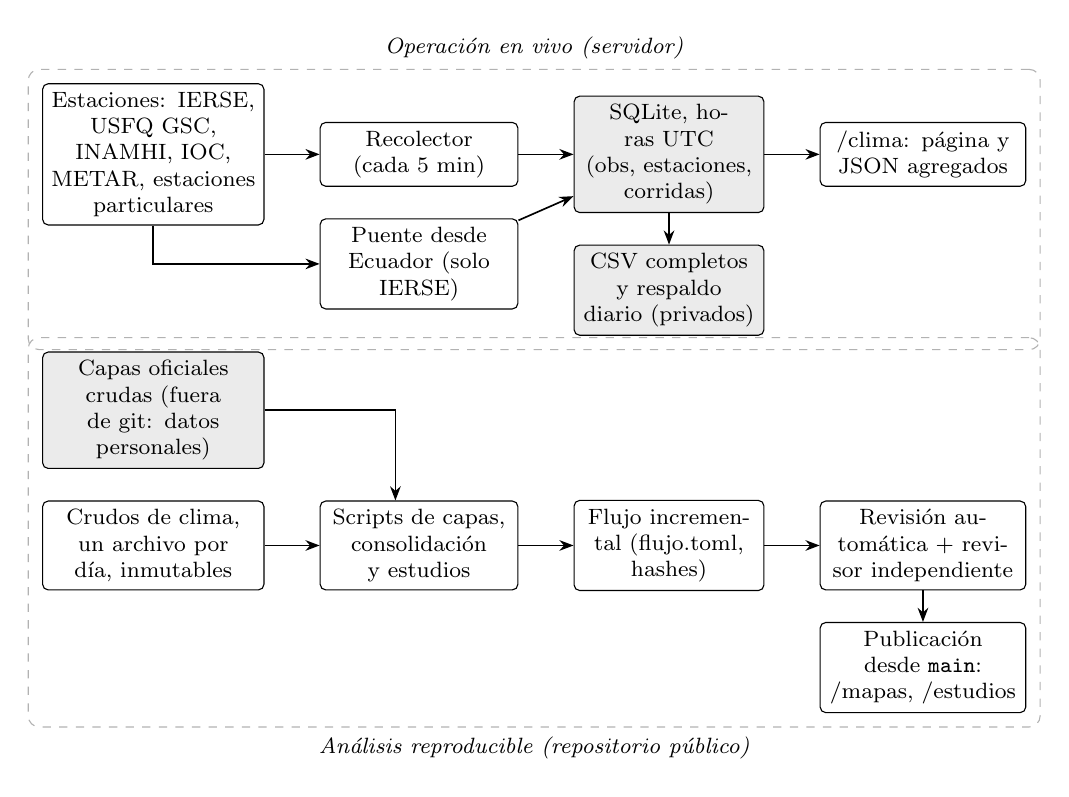
\begin{tikzpicture}[
      font=\footnotesize,
      caja/.style={draw, rounded corners=2pt, align=center, inner sep=3pt, minimum height=7mm, fill=white},
      priv/.style={caja, fill=black!8},
      flecha/.style={-{Stealth[length=1.8mm]}, semithick}]
    % carril en vivo
    \node[caja, text width=2.6cm] (fuentes) {Estaciones: IERSE, USFQ GSC, INAMHI, IOC, METAR, estaciones particulares};
    \node[caja, right=7mm of fuentes, text width=2.3cm] (rec) {Recolector\\(cada 5~min)};
    \node[caja, below=4mm of rec, text width=2.3cm] (puente) {Puente desde Ecuador (solo IERSE)};
    \node[priv, right=7mm of rec, text width=2.2cm] (db) {SQLite, horas UTC\\(obs, estaciones, corridas)};
    \node[caja, right=7mm of db, text width=2.4cm] (panel) {/clima: página y JSON agregados};
    \node[priv, below=4mm of db, text width=2.2cm] (csv) {CSV completos y respaldo diario (privados)};
    \draw[flecha] (fuentes) -- (rec);
    \draw[flecha] (fuentes.south) |- (puente);
    \draw[flecha] (puente) -- (db);
    \draw[flecha] (rec) -- (db);
    \draw[flecha] (db) -- (panel);
    \draw[flecha] (db) -- (csv);
    % carril reproducible
    \node[priv, below=16mm of fuentes, text width=2.6cm] (desc) {Capas oficiales crudas (fuera de git: datos personales)};
    \node[caja, below=4mm of desc, text width=2.6cm] (crudos) {Crudos de clima, un archivo por día, inmutables};
    \node[caja, right=7mm of crudos, text width=2.3cm] (scripts) {Scripts de capas, consolidación y estudios};
    \node[caja, right=7mm of scripts, text width=2.2cm] (flujo) {Flujo incremental (flujo.toml, hashes)};
    \node[caja, right=7mm of flujo, text width=2.4cm] (rev) {Revisión automática + revisor independiente};
    \node[caja, below=4mm of rev, text width=2.4cm] (pub) {Publicación desde \texttt{main}: /mapas, /estudios};
    \draw[flecha] (desc.east) -| ([xshift=-3mm]scripts.north);
    \draw[flecha] (crudos) -- (scripts);
    \draw[flecha] (scripts) -- (flujo);
    \draw[flecha] (flujo) -- (rev);
    \draw[flecha] (rev) -- (pub);
    \begin{scope}[on background layer]
      \node[draw=black!30, dashed, rounded corners, fit=(fuentes)(rec)(puente)(db)(panel)(csv), inner sep=5pt, label={[font=\footnotesize\itshape]above:Operación en vivo (servidor)}] {};
      \node[draw=black!30, dashed, rounded corners, fit=(desc)(crudos)(scripts)(flujo)(rev)(pub), inner sep=5pt, label={[font=\footnotesize\itshape]below:Análisis reproducible (repositorio público)}] {};
    \end{scope}
  \end{tikzpicture}
  \caption{Arquitectura de la infraestructura de datos de SOS Galápagos. En gris, lo que no se publica. No se muestran direcciones, servicios de las fuentes ni configuración de los servidores.}
  \label{fig:arquitectura}
\end{figure}

\begin{table}[ht]
  \centering\small
  \caption{Tipos de archivo del repositorio y regla que los gobierna (\texttt{CONTRIBUIR.md}, §1).}
  \label{tab:tipos}
  \begin{tabularx}{\linewidth}{l>{\raggedright\arraybackslash}X>{\raggedright\arraybackslash}X}
    \toprule
    Tipo & Ejemplos & Regla \\
    \midrule
    Fuente (se edita a mano) & scripts, manifiestos, textos de los estudios, código del recolector, documentación & se cambia en una rama y entra por \emph{pull request} \\
    \addlinespace
    Crudo externo (se descarga) & capas oficiales en \texttt{geodatos/descargas/}; crudos de clima en \texttt{clima/datos/<fuente>/crudos/} & las capas oficiales crudas no van a git (pesan ${\approx}\,400$~MB y traen datos personales); los crudos de clima sí, y nunca se modifican \\
    \addlinespace
    Generado (lo escribe un script) & capas finales, paquete del mapa, figuras, PDF, tablas consolidadas & nunca se edita a mano; ante un conflicto se toma la versión de \texttt{main} y se vuelve a correr el script \\
    \bottomrule
  \end{tabularx}
\end{table}

\subsection{Fuentes meteorológicas}
La tabla~\ref{tab:fuentes} resume las fuentes que entran al recolector. Solo se nombran: sus servicios de origen viven en una carpeta privada que no se versiona, y en el servidor, en la configuración del servicio.

\begin{table}[ht]
  \centering\small
  \caption{Fuentes meteorológicas y oceanográficas del recolector. Hora de origen tal como la marca la fuente; en la base todo se guarda en UTC.}
  \label{tab:fuentes}
  \begin{tabularx}{\linewidth}{l>{\raggedright\arraybackslash}Xll}
    \toprule
    Fuente & Estaciones & Paso & Hora de origen \\
    \midrule
    IERSE-WSN & 4 en Santa Cruz (Cerro Crocker, Santa Rosa, Los Guayabillos, Militar) & ${\approx}\,5$~min & UTC$-6$ \\
    USFQ GSC & 4 en San Cristóbal (El Junco, Cerro Alto, El Mirador, Merceditas) & 5~min & UTC$-5$ (aunque marque \enquote{Z}) \\
    INAMHI & M0191 Puerto Ayora, M0221 Puerto Baquerizo; respaldo horario de 90 días & 5~min / 1~h & UTC$-5$ \\
    IOC & mareógrafos de Puerto Ayora y Baltra & 5~min & UTC \\
    METAR & aeropuertos de Baltra y San Cristóbal & horario & UTC \\
    Estaciones particulares & WeatherLink en Puerto Ayora y Tempest en Punta Estrada & 5~min & UTC \\
    Modelos & nivel del mar y pronóstico de lluvia (Open-Meteo) & horario & según consulta \\
    \bottomrule
  \end{tabularx}
\end{table}

\subsection{Registros guardados en el repositorio}
\begin{itemize}
  \item \textbf{Crudos de IERSE-WSN}, en \path{clima/datos/ierse-wsn/crudos/AAAA-MM/AAAA-MM-DD.csv.gz}, tal como los entrega el servidor de origen (formato largo). Son 193 archivos diarios, del 23 de abril al 2 de noviembre de 2026, y ocupan 4,0~MB comprimidos. A partir de ellos se regeneran la serie de 5~min, la horaria y la diaria. La diaria incluye un porcentaje de cobertura (figura~\ref{fig:cobertura}).
  \item \textbf{Historial horario del INAMHI} del 16 de octubre al 2 de noviembre (\path{clima/datos/inamhi/historial/}). Se archivó porque la fuente borra lo que tiene más de 90 días: si no se guarda, es irrecuperable.
  \item \textbf{Series diarias de la FCD} de Puerto Ayora (desde 1965) y Bellavista, y \textbf{series horarias del UHSLC} de nivel del mar.
  \item \textbf{Capas geográficas} depuradas (\texttt{geodatos/capas/}), el paquete del mapa (\texttt{geodatos/export/}) y el entregable \texttt{mapas-galapagos/}, todo en EPSG:4326.
\end{itemize}
La base SQLite del servidor no está en el repositorio: las bases (\texttt{*.db}) están excluidas de git.

\begin{figure}[t]
  \centering
  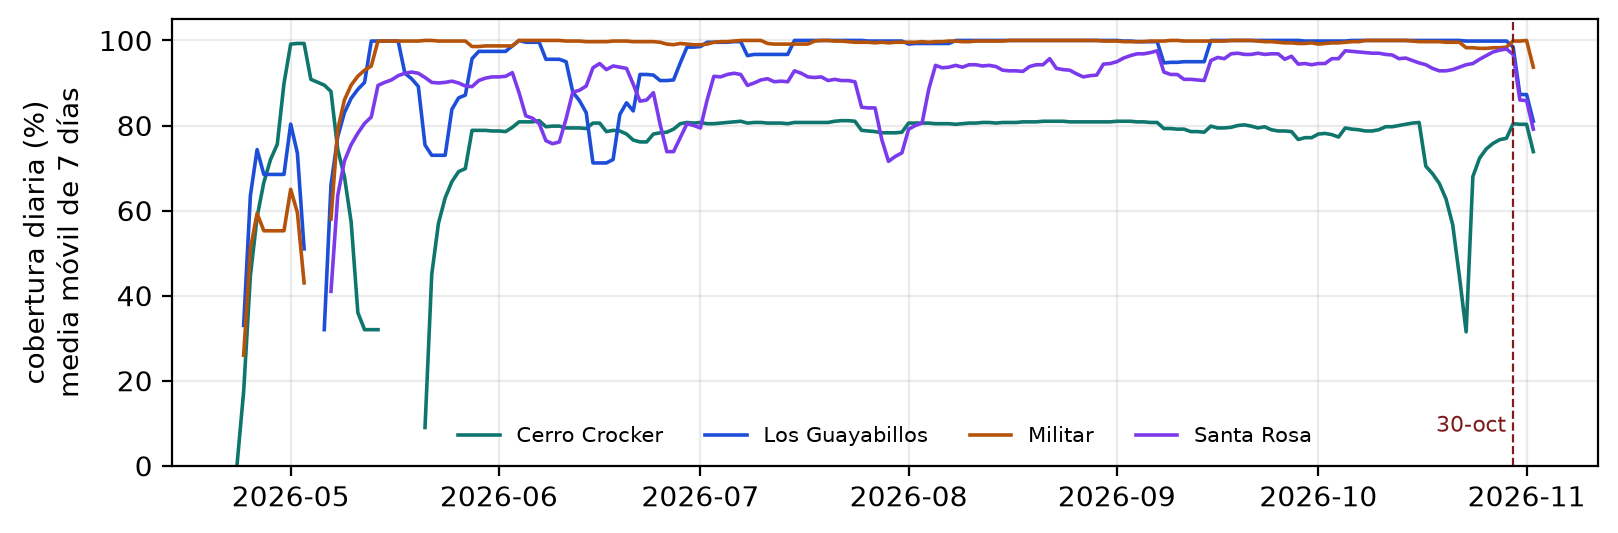
\includegraphics[width=\linewidth]{crudos.png}
  \caption{Cobertura diaria de las cuatro estaciones IERSE-WSN (porcentaje de los registros esperados cada 5~min, media móvil de 7 días), calculada desde las tablas consolidadas. Los huecos son días sin ningún registro. Cuando una estación no transmite, la lluvia de ese tramo no se mide: los totales de esos días son mínimos.}
  \label{fig:cobertura}
\end{figure}

% =====================================================================
\section{Métodos}

\subsection{Recolector}
El recolector es un programa en Python que un temporizador del sistema ejecuta cada 5~minutos. Cada fuente tiene su propia función, que convierte la hora de origen a UTC y escribe en tres tablas:
\begin{itemize}
  \item \texttt{obs}: una fila por fuente, estación, variable y hora (ISO~8601 en UTC), con clave primaria compuesta. Repetir una consulta no duplica datos.
  \item \texttt{estaciones}: los metadatos de cada estación.
  \item \texttt{corridas}: una fila por consulta, con su hora, la fuente, si tuvo éxito, el número de registros, la duración y el error, si lo hubo.
\end{itemize}
Una fuente caída no detiene a las demás: el error queda registrado en \texttt{corridas} y la corrida sigue.

La tabla \texttt{corridas} tiene además un uso operativo. Permite distinguir si una estación calló o si falló la recolección propia, y la regla de alerta solo trata como \enquote{silencio en alerta} el primer caso \citep{maya2026alerta}.

Para el INAMHI, las filas horarias de respaldo se guardan a la mitad de la hora y solo en las horas sin datos de 5~min. Así un corte se rellena sin duplicar lluvia. Las horas se guardan siempre en UTC. Galápagos está en UTC$-6$, pero INAMHI y GSC marcan la hora continental (UTC$-5$) aunque digan \enquote{Z}. Esa diferencia se comprobó con la hora actual y con el ciclo de la radiación solar. Un error de una hora en esta conversión movería todos los avisos.

\subsection{Puente de IERSE}
El servidor está fuera de Ecuador y el servicio de IERSE no le responde. Por eso, una máquina en Ecuador ejecuta cada 5~minutos el mismo recolector, solo para IERSE, sobre una base local. Después envía al servidor las filas nuevas por SSH, desde el último envío correcto más una hora de margen, con un mínimo de 2~h y un máximo de 72~h.

La llave del puente solo puede ejecutar una orden en el servidor: recibir filas. El receptor valida cada fila antes de guardarla. Solo acepta datos de IERSE, con identificadores, horas y valores bien formados, y sin caracteres que puedan inyectar contenido en la página. Si la llave se filtrara, no serviría para falsear la lluvia de otras fuentes.

Si la máquina duerme o se apaga, IERSE deja de actualizarse; al volver, recupera hasta 3 días.

\subsection{Publicación del panel de clima}
El recolector exporta un pequeño conjunto de JSON agregados para la página. El servidor web solo expone esa página y esos archivos: no hay descargas ni enlaces a las fuentes, y la página no se indexa. Los CSV mensuales completos se escriben cada hora en una carpeta privada, y la base se copia una vez al día. Las copias se conservan 14 días en el mismo servidor.

\subsection{Crudos inmutables y consolidación}
Los scripts de \texttt{clima/scripts/} bajan los días que faltan y los guardan sin correcciones. Los días con más de 2 días de antigüedad se consideran cerrados y no se vuelven a pedir; hoy y ayer se piden en cada corrida, porque las estaciones transmiten con retraso. Un día se puede rehacer de forma explícita.

Los filtros de calidad no tocan nunca el crudo: se aplican en la consolidación o en el análisis. Así, un error de filtrado se corrige volviendo a correr un script, sin perder el dato original.

\subsection{Flujo incremental}\label{sec:flujo}
Los estudios y las capas de estudios de \emph{/mapas} se rehacen con un flujo incremental (\path{geodatos/flujo.toml} y \path{geodatos/scripts/flujo.py}), en la tradición de \texttt{make} \citep{feldman1979} y de los gestores de flujos científicos \citep{koster2012}.

\paragraph{Declaración.} Cada paso $p$ declara:
\begin{itemize}
  \item su script y sus comandos;
  \item un conjunto de patrones de entrada $E_p$ (con comodines y grupos con nombre) y de salida $S_p$;
  \item los demás scripts que importa;
  \item marcas opcionales: \emph{pesado} (modelo 2D), \emph{red} (baja datos), \emph{manual} o \emph{siempre} (controles).
\end{itemize}

\paragraph{Grafo.} Un paso $p$ depende de otro $q$ si lee algo que $q$ escribe:
\begin{equation}\label{eq:dep}
  q \rightarrow p \iff \operatorname{arch}(E_p \cup C_p) \cap \operatorname{arch}(S_q) \neq \varnothing,
\end{equation}
donde $C_p$ son los scripts del paso y $\operatorname{arch}(\cdot)$ son los archivos que casan con los patrones. Cuando un patrón aún no tiene archivos, se compara por la forma del patrón. El orden de ejecución es un orden topológico del grafo \citep{kahn1962}, y un ciclo detiene el flujo con un mensaje.

\paragraph{Qué se rehace.} Para cada paso se guarda la huella de su última corrida correcta: el hash BLAKE2b del contenido de cada entrada y de cada script, y una firma de la propia declaración. Un paso se rehace en cinco casos:
\begin{itemize}
  \item cambió el contenido de una entrada;
  \item apareció o desapareció un archivo de entrada;
  \item falta una salida;
  \item cambió su declaración;
  \item se rehace un paso del que depende.
\end{itemize}
El hash se recalcula solo si cambian el tamaño o la fecha del archivo. Que se mire el contenido y no la fecha evita rehacer por un archivo que solo se copió.

\paragraph{Uso.} El modo \texttt{--seco} lista qué se rehace y por qué, sin ejecutar nada. Con \texttt{--cambio RUTA} responde \enquote{¿qué se rehace si cambia este archivo?}. Los pasos pesados, los que usan red y los manuales solo corren si se piden de forma explícita. Si el flujo falla en un paso, conserva el estado de los pasos que sí terminaron. Este modelo de dependencias se parece al de los sistemas de construcción con verificación por contenido \citep{mokhov2018}. La figura~\ref{fig:grafo} dibuja la reducción transitiva del grafo \citep{aho1972}.

\subsection{Revisión antes de publicar}
\texttt{geodatos/scripts/revisar\_publicacion.py} revisa el sitio generado y las fuentes versionadas. Si encuentra un error, la publicación se detiene (tabla~\ref{tab:revision}). El control de secretos lee los valores privados de las fuentes para buscarlos en lo publicado y en lo versionado, pero nunca los imprime.

El control de datos personales busca correos, teléfonos con formato ecuatoriano y números de cédula que pasan el dígito verificador. También busca, en las descargas, campos con nombres de contacto (teléfono, correo, propietario, representante\ldots). El control de cifras compara una lista de cifras clave de los textos con los datos de los que salen; si los datos cambian y el texto no, la revisión falla.

\begin{table}[ht]
  \centering\small
  \caption{Controles de la revisión automática (\texttt{revisar\_publicacion.py}) y lo que queda para el revisor humano o agente (\texttt{geodatos/estudios/PUBLICAR.md}).}
  \label{tab:revision}
  \begin{tabularx}{\linewidth}{l>{\raggedright\arraybackslash}X}
    \toprule
    Control & Qué comprueba \\
    \midrule
    1. Frescura & el sitio es más nuevo que sus textos, figuras y pendientes \\
    2. Enlaces & enlaces internos, anclas, imágenes, capas del mapa y vista 3D (externos, a pedido) \\
    3. Secretos & ni servicios de origen ni identificadores o credenciales de las fuentes meteorológicas \\
    4. Palabras & \enquote{refugio}, nunca \enquote{albergue}; \enquote{preliminar} solo en la etiqueta \\
    5. Voz & sin recomendaciones en voz de la universidad \\
    6. Datos personales & correos, teléfonos, cédulas y campos de contacto en páginas y descargas \\
    7. Pie & responsable y etiqueta \enquote{Datos preliminares} en cada página \\
    8. Cifras & las cifras clave de los textos coinciden con los datos \\
    9. Pendientes & la caché de issues y las páginas de pendientes coinciden \\
    10. Git & lo publicado corresponde a un commit (error en modo estricto) \\
    \midrule
    Revisor & que cada cifra nueva salga de un dato; conclusiones y confianza; tono; modelo frente a dato oficial; figuras, mapa y 3D en el navegador \\
    \bottomrule
  \end{tabularx}
\end{table}

La publicación solo se hace desde la rama \texttt{main}, con el árbol limpio y con un único script (\texttt{servidores/publicar.sh}), que deja en el servidor un archivo con el commit publicado. Después de publicar, el modo \texttt{--produccion} descarga cada página y la compara con la versión local.

\subsection{Comité de agentes de IA y revisión independiente}
Los estudios los elaboró un sistema de IA (Claude, de Anthropic) organizado como comité de agentes con papeles separados:
\begin{itemize}
  \item un asesor principal de hidrología e hidráulica;
  \item especialistas en meteorología, gestión del riesgo de desastres y planificación urbana y drenaje;
  \item un hidrólogo dedicado a San Cristóbal.
\end{itemize}
Un agente coordinador integra el trabajo. Las discrepancias se resolvieron de forma explícita y quedaron escritas. Algunos ejemplos:
\begin{itemize}
  \item el volumen del vaso de La Cascada (55\,000 frente a 125\,000~m³);
  \item el tiempo de concentración;
  \item el huso de los datos de modelos (UTC$-5$ frente a UTC$-6$);
  \item cifras sin fuente, que se retiraron.
\end{itemize}
Un revisor científico independiente revisó la versión de La Cascada.

\texttt{PUBLICAR.md} formaliza cinco papeles: responsable, asesor de producción, especialistas temáticos, revisor independiente y revisión automática. Solo el responsable publica. El revisor no puede ser quien escribió el cambio, y su visto bueno queda en el commit con una línea \texttt{Revisado-por}.

Las sesiones de agentes trabajan en paralelo, cada una en su rama y en su propia copia del repositorio (\emph{worktree}). Siguen reglas duras escritas en \texttt{AGENTS.md}:
\begin{itemize}
  \item no subir capas oficiales crudas, credenciales ni bases de datos;
  \item no publicar servicios de las fuentes;
  \item depurar los datos personales en el script;
  \item distinguir modelo de dato oficial;
  \item no editar archivos generados;
  \item no desplegar sin pedido.
\end{itemize}
Esta misma serie de informes se redactó así, con varias sesiones en paralelo sobre carpetas separadas.

\subsection{Gobernanza: issues, prioridades y dueños}
Lo pendiente vive solo como issues del repositorio, con una prioridad y un tipo:
\begin{itemize}
  \item \textbf{prioridad:} P1 (cambia decisiones de esta emergencia), P2 o P3;
  \item \textbf{tipo:} datos faltantes, más resolución, procesos, plataforma o gobernanza.
\end{itemize}
Las páginas de pendientes de \emph{/estudios} se generan desde esos issues, sin los de plataforma, y nunca se editan a mano. Cada carpeta tiene un dominio dueño: capas base, publicación de mapas, estudios, clima, entregable o servidores. Los archivos que toca casi todo el mundo (el manifiesto de capas, el índice de estudios y el README) se editan solo por bloque propio.

\subsection{Protocolo de datos personales}
Las capas oficiales de la SNGR y del MSP traen nombres y teléfonos de responsables de refugios y de fuentes de eventos. El protocolo tiene cuatro capas:
\begin{enumerate}
  \item las descargas crudas no entran en git;
  \item el script que produce cada capa copia solo una lista explícita de campos (lista blanca, en \texttt{07\_oficiales.py}), así que un campo nuevo de la fuente no se publica por omisión;
  \item las descripciones libres de los eventos de la SNGR, que traen nombres de personas afectadas, no se publican;
  \item la revisión automática busca contactos en todo lo que se publica.
\end{enumerate}
Nunca se nombra a personas afectadas. Las estaciones de particulares se presentan como \enquote{estación particular}, salvo autorización expresa del titular. La población se publica solo de forma agregada. El protocolo formal frente a la Ley Orgánica de Protección de Datos Personales \citep{lopdp2021} sigue abierto (\issue{48}). Las guías de responsabilidad de datos en la acción humanitaria \citep{iasc2021} son un marco de referencia para cerrarlo.

\subsection{Licencias por fuente}\label{sec:licencias}
El código propio se publica bajo Apache~2.0, con un aviso de atribución obligatorio. Los textos, las figuras, las capas y los resultados de los modelos propios se publican bajo CC~BY~4.0, con atribución a la USFQ. Los datos de terceros conservan su licencia, y si esa licencia es más restrictiva, prevalece (tabla~\ref{tab:licencias}).

\begin{table}[ht]
  \centering\small
  \caption{Licencias de las fuentes de terceros y su efecto en lo derivado (\texttt{LICENCIA-DATOS.md}, \texttt{mapas-galapagos/documentacion/03-fuentes-y-licencias.md}).}
  \label{tab:licencias}
  \begin{tabularx}{\linewidth}{>{\raggedright\arraybackslash}p{3.6cm}>{\raggedright\arraybackslash}p{3.2cm}>{\raggedright\arraybackslash}X}
    \toprule
    Fuente & Licencia & Efecto en lo derivado \\
    \midrule
    OpenStreetMap & ODbL 1.0 & las bases derivadas se publican bajo ODbL \\
    Copernicus GLO-30 & libre con atribución & texto de atribución fijo \\
    Google Open Buildings v3 & CC BY 4.0 (u ODbL) & atribución \\
    IGM, CGREG, SNGR, INOCAR, INEC, MSP, MINEDUC, CONALI & información pública con cita & citar a la institución; confirmar para usos formales \\
    IERSE-WSN \citep{orellana2023} & CC BY-NC-ND 4.0 & sin uso comercial ni obras derivadas: los modelos con su lluvia requieren permiso del titular \\
    FCD, series climáticas & CC BY-NC-SA & lo derivado (p.\,ej., curvas IDF), no comercial y con la misma licencia \\
    USFQ GSC & no declarada (\issue{46}) & sus series no se redistribuyen \\
    Proyecto DARWIN (U.~de Marburgo) & acuerdo que prohíbe redistribuir (\issue{76}) & solo metadatos y DOI \\
    GAR (TU Berlín), Open-Meteo & CC BY 4.0 & atribución \\
    \bottomrule
  \end{tabularx}
\end{table}

% =====================================================================
\section{Resultados: estado de la infraestructura}

\subsection{El grafo del flujo}
El 4 de noviembre, \texttt{flujo.toml} declara 35 pasos que usan 31 scripts distintos (tabla~\ref{tab:flujo}, figura~\ref{fig:grafo}). Por tipo:
\begin{itemize}
  \item 25 pasos normales;
  \item 7 pesados: modelos 2D de Santa Cruz y San Cristóbal, sensibilidad, tormentas sintéticas, sus figuras y curvas IDF. Uno de ellos, el contraste con ANUGA, es además manual;
  \item 2 que bajan datos de internet: lluvia de modelos e issues;
  \item 1 control que corre siempre: la revisión.
\end{itemize}
Las 92 dependencias se reducen a 54 aristas sin las transitivas, repartidas en 8 niveles. El paso que genera el sitio web depende directamente de 28 pasos.

\begin{figure}[t]
  \centering
  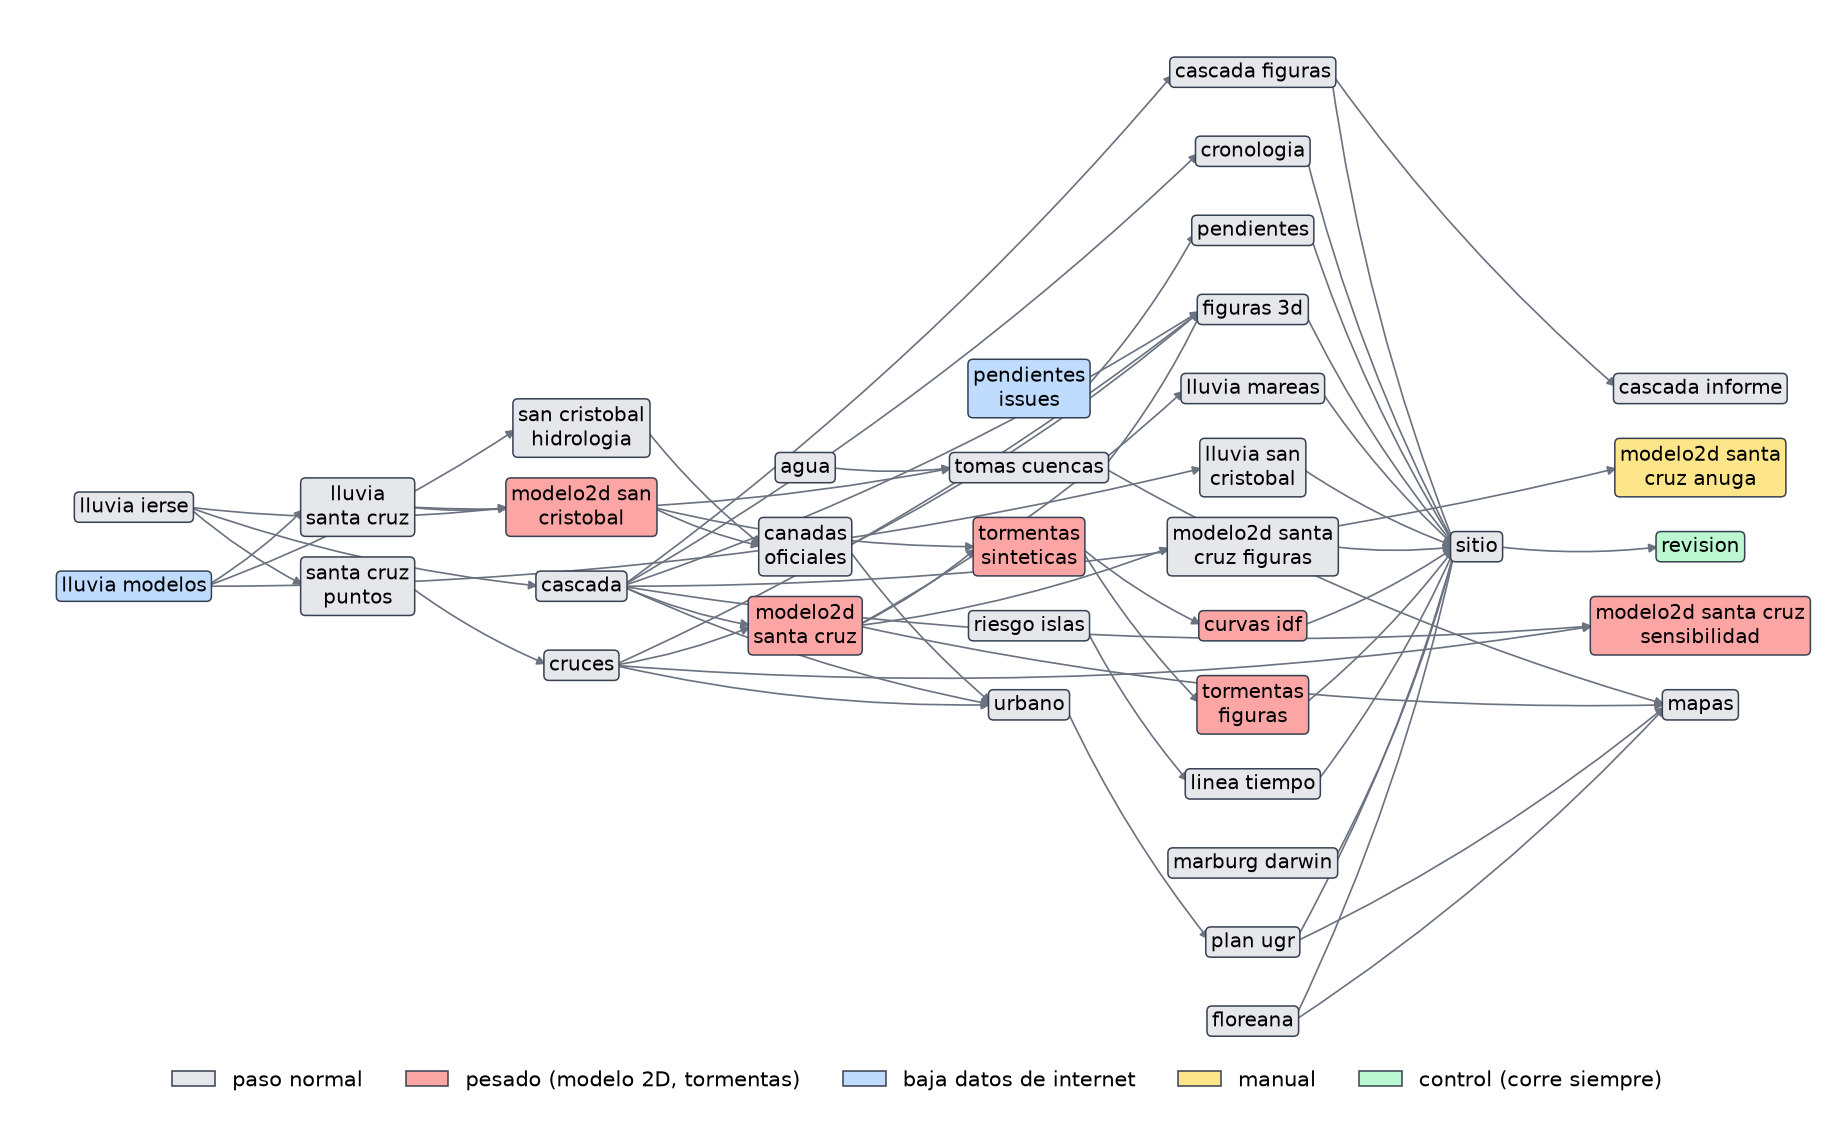
\includegraphics[width=\linewidth]{flujo_grafo.png}
  \caption{Grafo del flujo incremental de los estudios (reducción transitiva: 54 de 92 dependencias). Cada paso queda a la izquierda del primero que usa sus salidas. Generado desde \texttt{geodatos/flujo.toml} con las funciones de \texttt{flujo.py}, sin ejecutar ningún paso.}
  \label{fig:grafo}
\end{figure}

\begin{table}[ht]
  \centering\small
  \caption{Alcance de cambios típicos: pasos que leen directamente el archivo y total de pasos que se rehacen al propagar el cambio por el grafo (de 35).}
  \label{tab:flujo}
  \begin{tabularx}{\linewidth}{>{\raggedright\arraybackslash}Xccc}
    \toprule
    Archivo que cambia & Directos & Total & Pesados \\
    \midrule
    Serie de 5~min de IERSE (\texttt{serie\_5min.csv.gz}) & 6 & 27 & 7 \\
    DEM de Santa Cruz & 12 & 22 & 6 \\
    Serie diaria de la FCD (Bellavista) & 2 & 4 & 1 \\
    Caché de issues (\texttt{pendientes.json}) & 1 & 3 & 0 \\
    Un texto del estudio de Santa Cruz & 1 & 2 & 0 \\
    \bottomrule
  \end{tabularx}
\end{table}

Una nueva descarga de lluvia de IERSE alcanza 27 de los 35 pasos, entre ellos los 7 pesados. Eso cuantifica el costo de rehacer los estudios cada vez que llega un día nuevo, y justifica que los pesados solo corran a pedido. Un texto corregido, en cambio, solo regenera el sitio y vuelve a pasar la revisión.

\subsection{Crudos y cobertura}
Los crudos de IERSE cubren 193 días: 8 de abril, entre 30 y 31 por mes de mayo a octubre, y 2 de noviembre. La cobertura media diaria es:
\begin{itemize}
  \item Militar: 98,2\,\% (184 días con datos);
  \item Los Guayabillos: 95,6\,\% (181 días);
  \item Santa Rosa: 90,3\,\% (180 días);
  \item Cerro Crocker: 78,4\,\% (174 días).
\end{itemize}
Cerro Crocker se queda en ${\approx}\,80$\,\% desde junio y su pluviómetro parece obstruido desde agosto (figura~\ref{fig:cobertura}; \issue{56}). El 30-oct, las estaciones dejaron de transmitir a las 21:22--21:25 y volvieron unas 21~h después. Esa lluvia no está en los crudos, y su recuperación es un pendiente P1 (\issue{62}).

\subsection{Pendientes de gobernanza y plataforma}
El 4 de noviembre hay 81 issues, todos abiertos: 35 de prioridad P1, 36 de P2 y 10 de P3. La tabla~\ref{tab:issues} resume los de gobernanza y plataforma que tocan esta infraestructura.

\begin{table}[ht]
  \centering\small
  \caption{Issues de gobernanza y plataforma relacionados con la infraestructura (todos abiertos el 4-nov-2026).}
  \label{tab:issues}
  \begin{tabularx}{\linewidth}{lc>{\raggedright\arraybackslash}X}
    \toprule
    Issue & Prioridad & Tema \\
    \midrule
    \issue{38} & P1 & respaldo de la base del clima fuera del servidor (hoy, copias locales de 14 días) \\
    \issue{39} & P1 & aviso si el recolector deja de correr \\
    \issue{45} & P1 & acuerdos de intercambio de datos con GAD, CGREG, DPNG, FCD, INAMHI, SNGR e INOCAR \\
    \issue{48} & P1 & protocolo de datos personales (LOPDP) \\
    \issue{49} & P1 & distinguir siempre dato oficial de modelo propio \\
    \issue{76} & P1 & series del proyecto DARWIN y permiso para publicar derivados \\
    \issue{36} & P2 & publicación automática desde \texttt{main} \\
    \issue{37} & P2 & validación automática en cada \emph{pull request} (GeoJSON, EPSG:4326, datos personales, catálogo) \\
    \issue{46} & P2 & licencia de los datos del GSC \\
    \issue{47}, \issue{42} & P2 & metadatos y catálogo por capa (fuente, fecha, licencia, resolución, responsable) \\
    \issue{50} & P2 & licencia del código y de los datos derivados \\
    \issue{51} & P2 & equipo local (USFQ, GAD, CGREG) que mantenga los datos después de la emergencia \\
    \issue{43}, \issue{44} & P3 & tamaño del repositorio; capas heredadas que dicen \enquote{albergue} \\
    \bottomrule
  \end{tabularx}
\end{table}

% =====================================================================
\section{Discusión y limitaciones}

\paragraph{Puntos únicos de falla.} La infraestructura tiene tres:
\begin{itemize}
  \item el puente de IERSE corre en una sola máquina personal: si se apaga más de 3 días, se pierde lluvia;
  \item la base del servidor solo tiene copias en el mismo servidor (\issue{38});
  \item nada avisa si el recolector deja de correr (\issue{39}).
\end{itemize}
Una caída de cualquiera de los tres en plena tormenta repetiría el problema del 30-oct, cuando los datos faltaron justo en el peor momento. La regla de alerta distingue el silencio de una estación del fallo propio, pero solo si la tabla de corridas existe y está al día.

\paragraph{El flujo es tan bueno como sus declaraciones.} El grafo de dependencias sale de lo que cada paso \emph{declara} leer y escribir. Si un script lee un archivo que no está declarado, el flujo no lo rehace cuando ese archivo cambia, y el resultado queda desactualizado sin aviso. La revisión de frescura solo mira las fuentes del sitio, no los datos intermedios. Además, el estado de las corridas es local, así que cada copia del repositorio empieza por dar por buenas las salidas versionadas (\texttt{--marcar}).

\paragraph{Reproducibilidad parcial.} Cualquiera puede rehacer los estudios desde los crudos de clima y las capas versionadas. Las capas base, en cambio, se rehacen desde descargas que no están en git (${\approx}\,400$~MB, con datos personales), y algunas fuentes tienen servicios que cambian o datos que caducan: el INAMHI guarda solo 90 días. Archivar los crudos en cuanto llegan mitiga lo segundo. No hay, por ahora, un depósito con DOI de cada versión publicada.

\paragraph{Licencias que no encajan.} El contenido propio se publica bajo CC~BY~4.0, pero la lluvia de IERSE es CC~BY-NC-ND, y casi todos los modelos de Santa Cruz la usan. Mientras no haya permiso escrito del titular, las salidas de esos modelos quedan sujetas a esa restricción. Algo parecido pasa con el GSC (licencia no declarada) y con DARWIN (redistribución prohibida). El issue \issue{50} pide definir las licencias propias. En la práctica ya se adoptaron Apache~2.0 y CC~BY~4.0, pero el issue sigue abierto.

\paragraph{Agentes de IA.} El comité de agentes permitió tener en cuatro días estudios con cientos de cifras trazables a un script. A cambio:
\begin{itemize}
  \item ningún estudio tiene revisión de profesionales habilitados ni visita de campo;
  \item el revisor independiente también es, en general, un agente;
  \item la línea \texttt{Revisado-por} que pide \texttt{PUBLICAR.md} no aparece todavía en el historial de esta rama de trabajo.
\end{itemize}
La revisión automática atrapa lo que un programa puede ver, como los secretos, los datos personales y las cifras clave. El tono, las conclusiones y la distinción entre modelo y dato oficial dependen del revisor.

\paragraph{Seguridad.} No publicar servicios de las fuentes ni la configuración de los servidores reduce la superficie expuesta, pero no la elimina. El control de secretos busca valores conocidos; un secreto nuevo que no esté en la carpeta privada pasaría inadvertido. Si un secreto llega a un commit, la única corrección posible es limpiar el historial y cambiar la credencial.

% =====================================================================
\section{Conclusiones y trabajo futuro}
\begin{enumerate}
  \item La infraestructura separa operación en vivo (recolector, SQLite en UTC, panel con datos agregados) y análisis reproducible (crudos inmutables, scripts, flujo incremental). Los separa por diseño, no solo por carpetas.
  \item El flujo incremental hace explícitas las dependencias: 35 pasos y 92 dependencias. Así se sabe qué rehacer ante un dato nuevo; la lluvia de IERSE alcanza 27 pasos.
  \item La revisión automática y el revisor independiente cubren riesgos distintos: lo que un programa puede verificar y lo que requiere juicio.
  \item La privacidad se resuelve en el origen (lista blanca de campos, crudos fuera de git) y se verifica al publicar.
  \item Los mayores riesgos abiertos son los puntos únicos de falla (\issue{38}, \issue{39}), los acuerdos y licencias de datos (\issue{45}, \issue{46}, \issue{76}) y la continuidad después de la emergencia (\issue{51}).
\end{enumerate}

Trabajo pendiente (todo como issues):
\begin{itemize}
  \item respaldo externo y monitoreo del recolector (\issue{38}, \issue{39});
  \item validación en cada \emph{pull request} y publicación automática desde \texttt{main} (\issue{36}, \issue{37});
  \item catálogo de metadatos por capa (\issue{42}, \issue{47});
  \item protocolo LOPDP (\issue{48});
  \item acuerdos de datos y licencias pendientes (\issue{45}, \issue{46}, \issue{50}, \issue{76});
  \item equipo local que mantenga la infraestructura (\issue{51}).
\end{itemize}

\section*{Disponibilidad de datos y código}
{\small\raggedright Todo está en el repositorio público \emph{mayait/sosgalapagos-datos}, salvo los servicios de origen, las credenciales y la configuración de los servidores:
\begin{itemize}
  \item recolector: \texttt{clima/recolector/} (\texttt{recolector.py}, \texttt{fuentes\_extra.py}); puente: \texttt{clima/puente/}; documentación: \texttt{clima/LEEME.md} y \texttt{servidores/README.md};
  \item crudos y tablas: \texttt{clima/datos/} (\texttt{LEEME.md} con la forma de citar cada fuente);
  \item flujo: \texttt{geodatos/flujo.toml} y \texttt{geodatos/scripts/flujo.py}; revisión: \texttt{geodatos/scripts/revisar\_publicacion.py} y \texttt{geodatos/estudios/PUBLICAR.md};
  \item reglas: \texttt{AGENTS.md}, \texttt{CONTRIBUIR.md}, \texttt{LICENCIA-DATOS.md}, \texttt{CITATION.cff};
  \item figuras~\ref{fig:cobertura} y~\ref{fig:grafo} y cifras de la sección de resultados: \texttt{informes/2026-10-infraestructura/figuras.py}, que escribe \texttt{figuras/resumen.json}.
\end{itemize}
Este informe se compila con \texttt{informes/compilar.sh 2026-10-infraestructura}.\par}

\bibliographystyle{sosg}
\bibliography{referencias,bib-2026-10}

\end{document}
